\section{Task and Dialog Analysis}
Another important phase is understanding how users interact with systems is crucial for designing intuitive and efficient interfaces. Task and dialog analysis are two fundamental methodologies that help designers and researchers dissect and understand user interactions, ultimately leading to better system design and user experience. Task analysis is a systematic approach to understanding the activities users perform to achieve their goals when using a system. This involves breaking down tasks into smaller, manageable components to study the user's workflow in detail. Task analysis helps identify user needs, uncover potential problems, and inform the design of user interfaces by ensuring they align with how users naturally perform tasks.\\
Dialog analysis focuses on the interaction between the user and the system, particularly the communication patterns and language used during this interaction. This analysis is crucial for designing systems that support effective and efficient communication, whether through graphical user interfaces, command-line interfaces, or voice-controlled systems.
One of the common techniques used in Human Computer Interaction is \textbf{Hierarchical Task Analysis (HTA)} focuses on decomposing tasks into sub-tasks and operations, creating a structured hierarchy that shows how each component contributes to achieving the overall goal. HTA breaks down tasks into sub-tasks and operations. It provides a clear visualization of the steps users take to achieve their goals, highlighting dependencies and sequences in the workflow. HTA is particularly useful for identifying redundant steps, optimizing processes, and ensuring that the design supports users' natural task flows.\\
To do this analysis step we also used \textbf{State Transition Network (STN)}, also known as State Transition Diagram or State Machine, which a graphical representation of a system that illustrates the different states a system can be in and how it transitions from one state to another based on user actions or events. It helps to demonstrate the flow of tasks, depicting how the system responds to user actions and transitions from one state to another, thereby facilitating a better understanding of the interaction dynamics and aiding in the optimization of task performance.
\subsection{Hierarchical Task Analysis (HTA)}
\subsubsection{Set custom notification}
This task is linked with the view document list and allows to change only the expiration settings without changing the other information of a document. 
\begin{figure}[H]
	\centering
	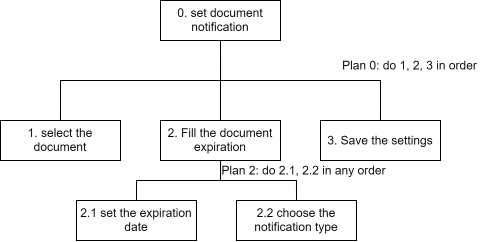
\includegraphics[width=\textwidth]{../Draw.io diagrams/set_notification.drawio.png}  % Replace 'example-image' with the filename of your image
	\caption{HTA for the requirement set custom notification}
\end{figure}
\subsubsection{Add a new document}
This is the classical way to add a document, this option allows the user to navigate on the file system of the device to upload the document on the remote repository.
The related HTA in the following picture explains better the details of this operation.
\begin{figure}[H]
	\centering
	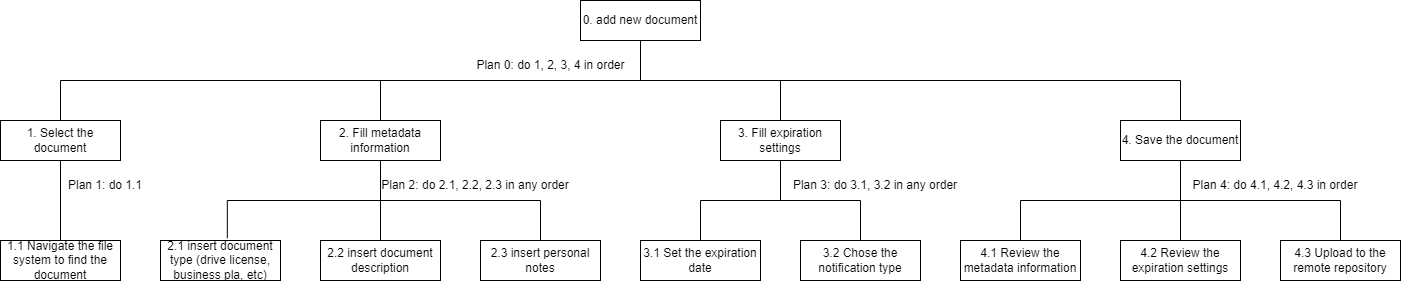
\includegraphics[width=\textwidth]{../Draw.io diagrams/add_new_document.drawio.png}  % Replace 'example-image' with the filename of your image
	\caption{HTA for the requirement Add new document}
\end{figure}
\subsubsection{Add a new document using the camera}
The system allows to upload of documents to be managed using the phone camera. With this feature is possible to load a document that is not digital and upload it in the remote repository. Then in the following picture is present the related HTA.
\begin{figure}[H]
	\centering
	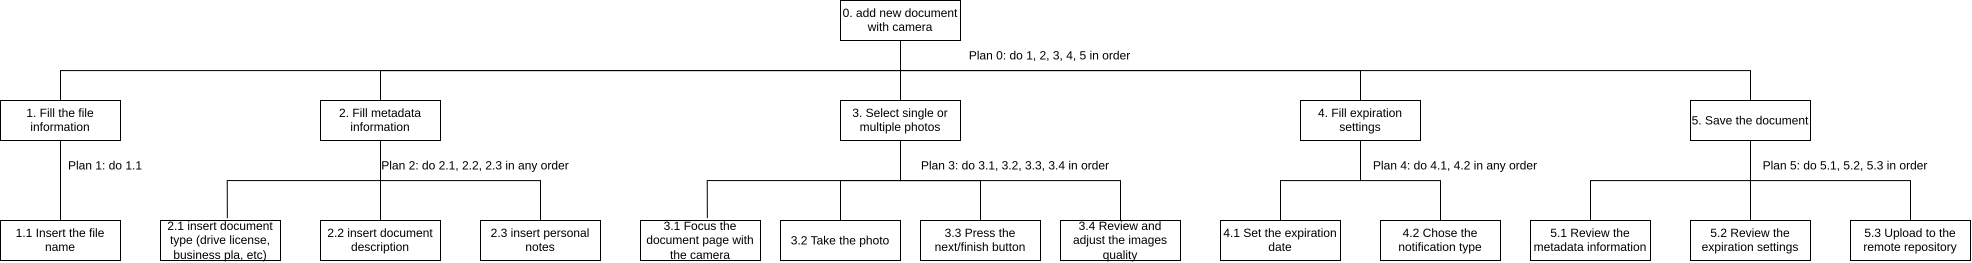
\includegraphics[width=\textwidth]{../Draw.io diagrams/add_new_document_camera.drawio.png}  % Replace 'example-image' with the filename of your image
	\caption{HTA for the requirement Add new document using the camera}
\end{figure}
\subsubsection{View document list}
This task allows the users to view all uploaded documents using the filters to adjust the search. It is possible to look for the metadata information, document information, and expiration dates.
\begin{figure}[H]
	\centering
	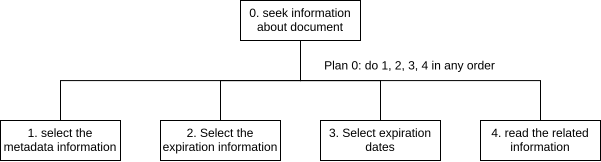
\includegraphics[width=\textwidth]{../Draw.io diagrams/search_and_view_documents.drawio.png}  % Replace 'example-image' with the filename of your image
	\caption{HTA for the requirement View documents list}
\end{figure}
\subsubsection{Edit an existing element}
This task allows the users to view all uploaded documents using the filters to adjust the search. It is possible to look for the metadata information, document information, and expiration dates.
\begin{figure}[H]
	\centering
	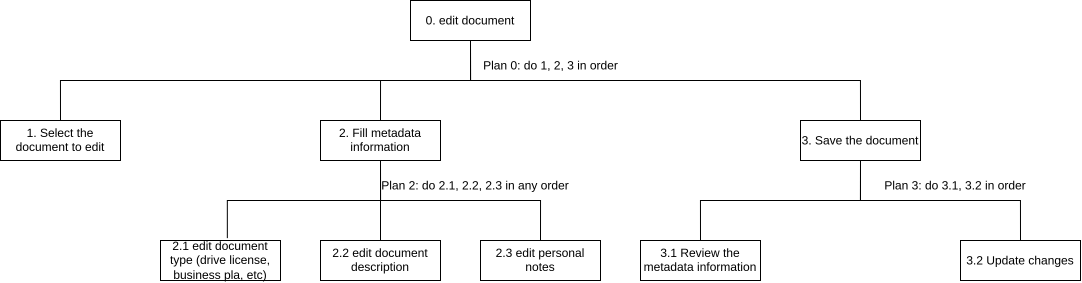
\includegraphics[width=\textwidth]{../Draw.io diagrams/edit_document.drawio.png}  % Replace 'example-image' with the filename of your image
	\caption{HTA for the requirement Edit an exisisting element}
\end{figure}
\subsubsection{Remove document}
This task is linked to the view document list and allows removal of a document from the system.
\begin{figure}[H]
	\centering
	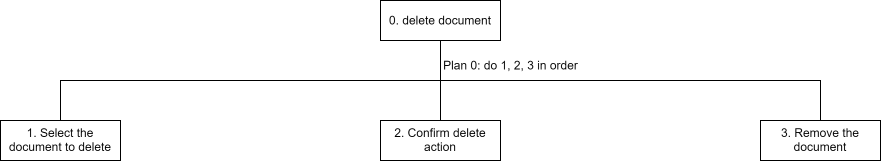
\includegraphics[width=\textwidth]{../Draw.io diagrams/delete_document.drawio.png}  % Replace 'example-image' with the filename of your image
	\caption{HTA for the requirement Remove documents}
\end{figure}
\subsection{State Transition Network (STN)}
In this section, we will examine the State Transition Network (STN) corresponding to the specific tasks previously analyzed through Hierarchical Task Analysis (HTA). The tasks and their significance remain unchanged from our earlier descriptions. However, this time we will focus on the interactions between the user and the system, detailing the dialogue that occurs during these tasks, including user actions and system responses.
\subsubsection{Add a new document}
This diagram covers the necessary steps and different states needed to add a document either from a saved file o scan it using the smartphone camera, add the document metadata, and adjust the expiration settings.
\begin{figure}[H]
	\centering
	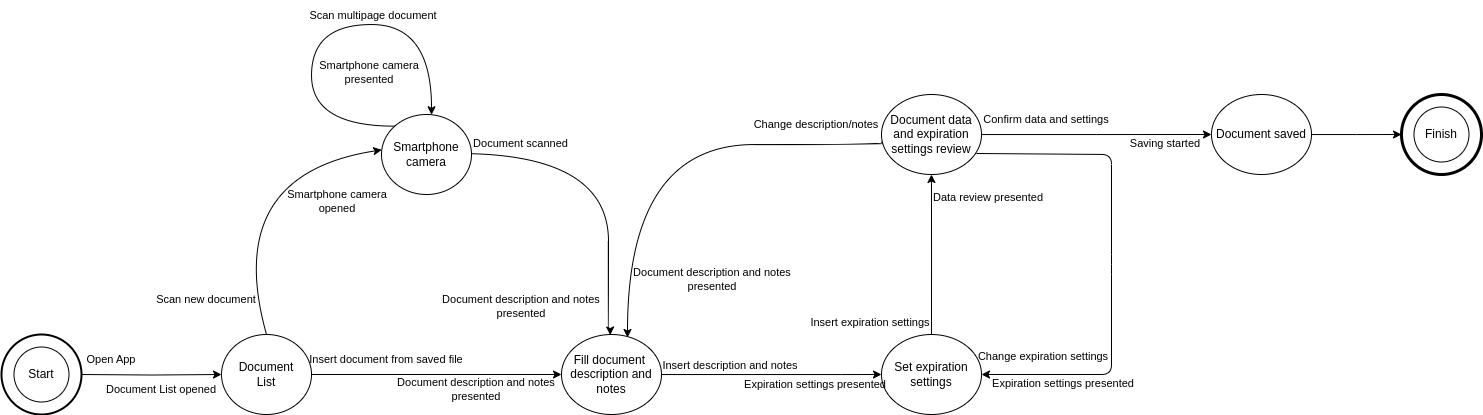
\includegraphics[width=\textwidth]{../Draw.io diagrams/documnet_add_STN.drawio.png}  % Replace 'example-image' with the filename of your image
	\caption{STN for add new document}
\end{figure}
\subsubsection{Edit document}
This diagram covers the necessary steps and different states needed to edit an existing document. It shows the different steps necessary to edit the document metadata and the expiration settings.
\begin{figure}[H]
	\centering
	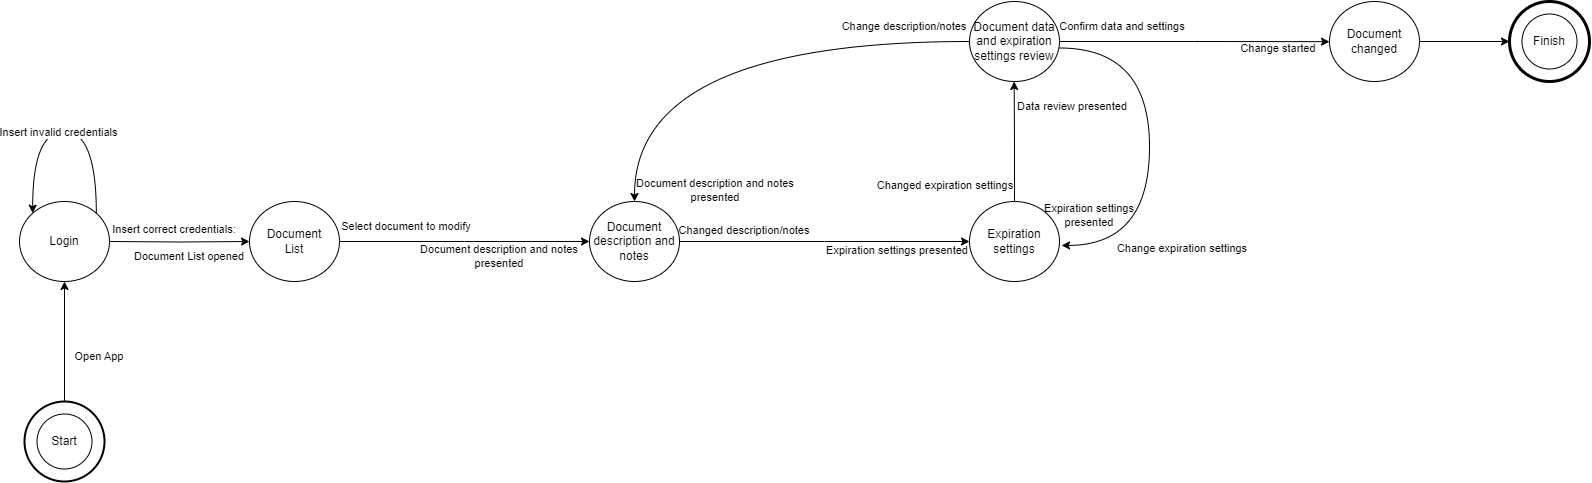
\includegraphics[width=\textwidth]{../Draw.io diagrams/document_edit_STN.drawio.png}  % Replace 'example-image' with the filename of your image
	\caption{STN for edit document}
\end{figure}
\subsubsection{Remove document}
This diagram shows the steps and different states necessary to delete an existing document.
\begin{figure}[H]
	\centering
	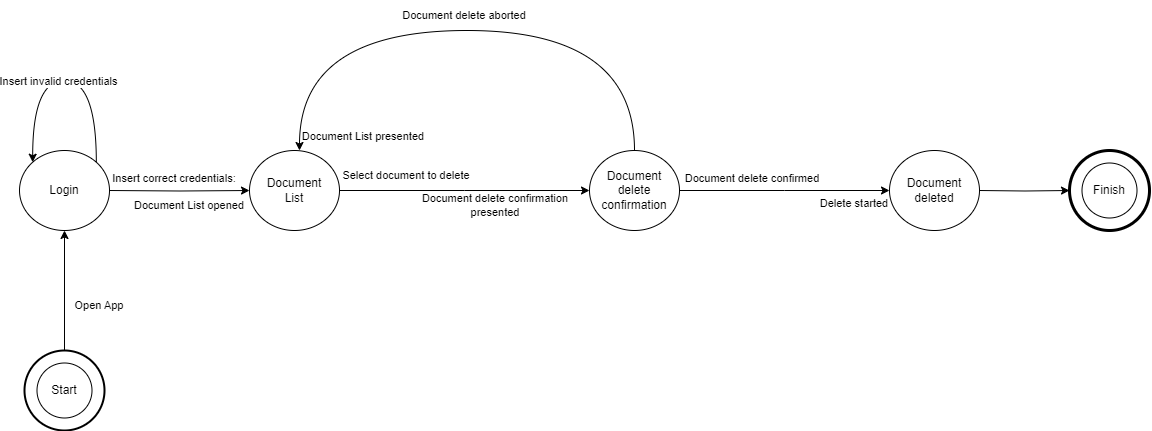
\includegraphics[width=\textwidth]{../Draw.io diagrams/document_delete_STN.drawio.png}  % Replace 'example-image' with the filename of your image
	\caption{STN for remove document}
\end{figure}
\subsubsection{View document list}
This diagram shows the steps and different states necessary to view and filter the list of available documents.
\begin{figure}[H]
	\centering
	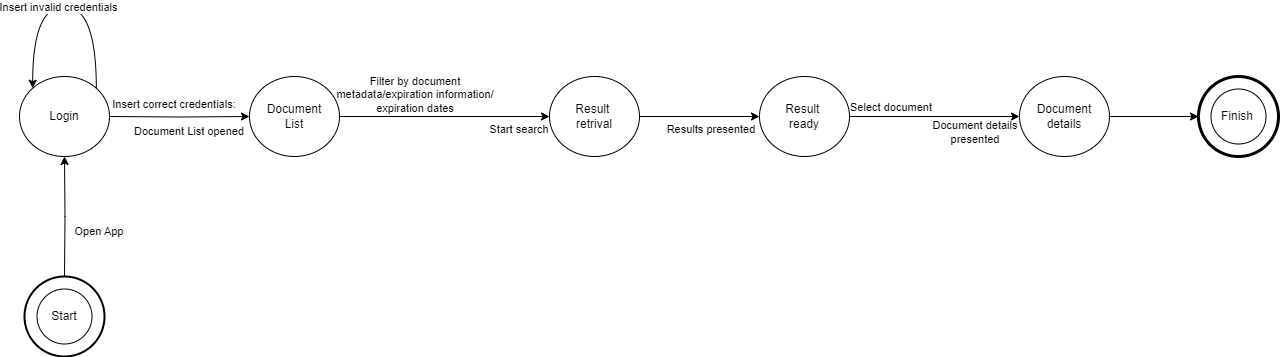
\includegraphics[width=\textwidth]{../Draw.io diagrams/document_search_STN.drawio.png}  % Replace 'example-image' with the filename of your image
	\caption{STN for view documents list}
\end{figure}
